\documentclass{standalone}
\usepackage{mintikz}

\begin{document}
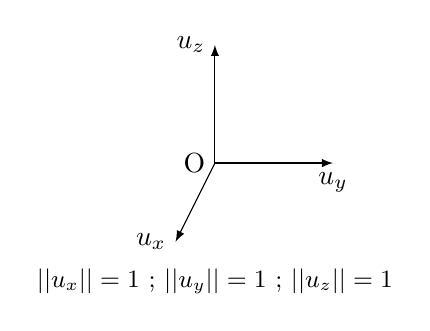
\begin{tikzpicture}[scale=1]  
    % \helpgrid{3}{3}
\draw [->,-latex] (0,0) --++ (-0.5,-1) node [left] {$\vv{u}_x$}	;   
\draw [->,-latex] (0,0) --++ (1.5,0) node [below] {$\vv{u}_y$}	;
\draw [->,-latex] (0,0) --++ (0,1.5) node [left] {$\vv{u}_z$}	; 
\node at (0,0) [left]{O};
\node at (0,-1.5) {\small $||\vv{u}_x||=1$ ; $||\vv{u}_y||=1$ ; $||\vv{u}_z||=1$};                      
\end{tikzpicture}                                      
\end{document}
